\section{Interfejs komunikacyjny}

Budowę interfejsu komunikacyjnego rozpoczęto od zaimplementowania modułów UART. Układ ich wyprowadzeń przedstawiono na Rys. \ref{uart-structure}. Wąskie strzałki symbolizują linie jednobitowe. Strzałki czerwone oraz żółte to linie wielobitowe. Pierwsze z~nich oznaczają, że są port skierowany jest do ``wewnątrz'' struktury urządzenia. Z~kolei w~przypadku drugich porty skierowane są ``na zewnątrz''. Konwencja ta została zachowana w~przypadku kolejnych rysunków.

Wejście \verb|clk| to podłączenie do głównego zegara systemowego, natomiast \verb|reset| to asynchroniczny reset układu (aktywny stanem niskim). Wejścia te są uniwersalne dla wszystkich implementowanych modułów. Porty \verb|rate| pozwalają określić szybkość transmisji. Wyrażana jest ona jako ilość cykli zegara systemowego przypadających na jeden znak wysyłany/transmitowany (minus 1). W~przypadku interfejsu odbierającego ustawienie wartości 0~na tym porcie zablokuje odbiór danych\footnote{Stan linii RX testowany jest w~połowie trwania znaku, co wymusza maksymalny stosunek prędkości transmisji do prędkości zegara systemowego na poziomie 1:2}. Oba moduły implementują także linię wyjściową \verb|busy|, która, gdy ustawiona w~stanie wysokim, oznacza, że układ zajęty jest odbiorem/transmisją danych. 

Podsystem odbiorczy udostępnia wyjście odebranych danych \verb|data| oraz oczywiście linię szeregową \verb|rx|. Port \verb|error| reprezentowany jest jako trzybitowa linia typu \verb|record|. Ustawiana jest w~momencie zmiany stanu linii \verb|busy| ze stanu wysokiego na niski i~zawiera flagi błędu odbioru bitu startu, bitów stopu oraz parzystości. Wystąpienie błędu sygnalizowane jest stanem wysokim. Równolegle z~flagami błędów ustawiany jest również port \verb|data|\footnote{W~przypadku wystąpienia błędu odbioru port \textit{data} jest zerowany}. Podsystem nadawczy posiada porty \verb|data| i~\verb|tx| o~znaczeniu analogicznym do przypadku odbiorczego. Udostępnia on także linię \verb|transfer|. Ustawienie jej w~stan wysoki\footnote{Linia aktywna jest \underline{poziomem} wysokim} w~czasie, gdy linia \verb|busy| znajduje się w~stanie niskim, rozpoczyna transmisję danych znajdujących się na wejściu \verb|data|.

\vspace{0.5cm}
\begin{figure}[ht]
    \centering
    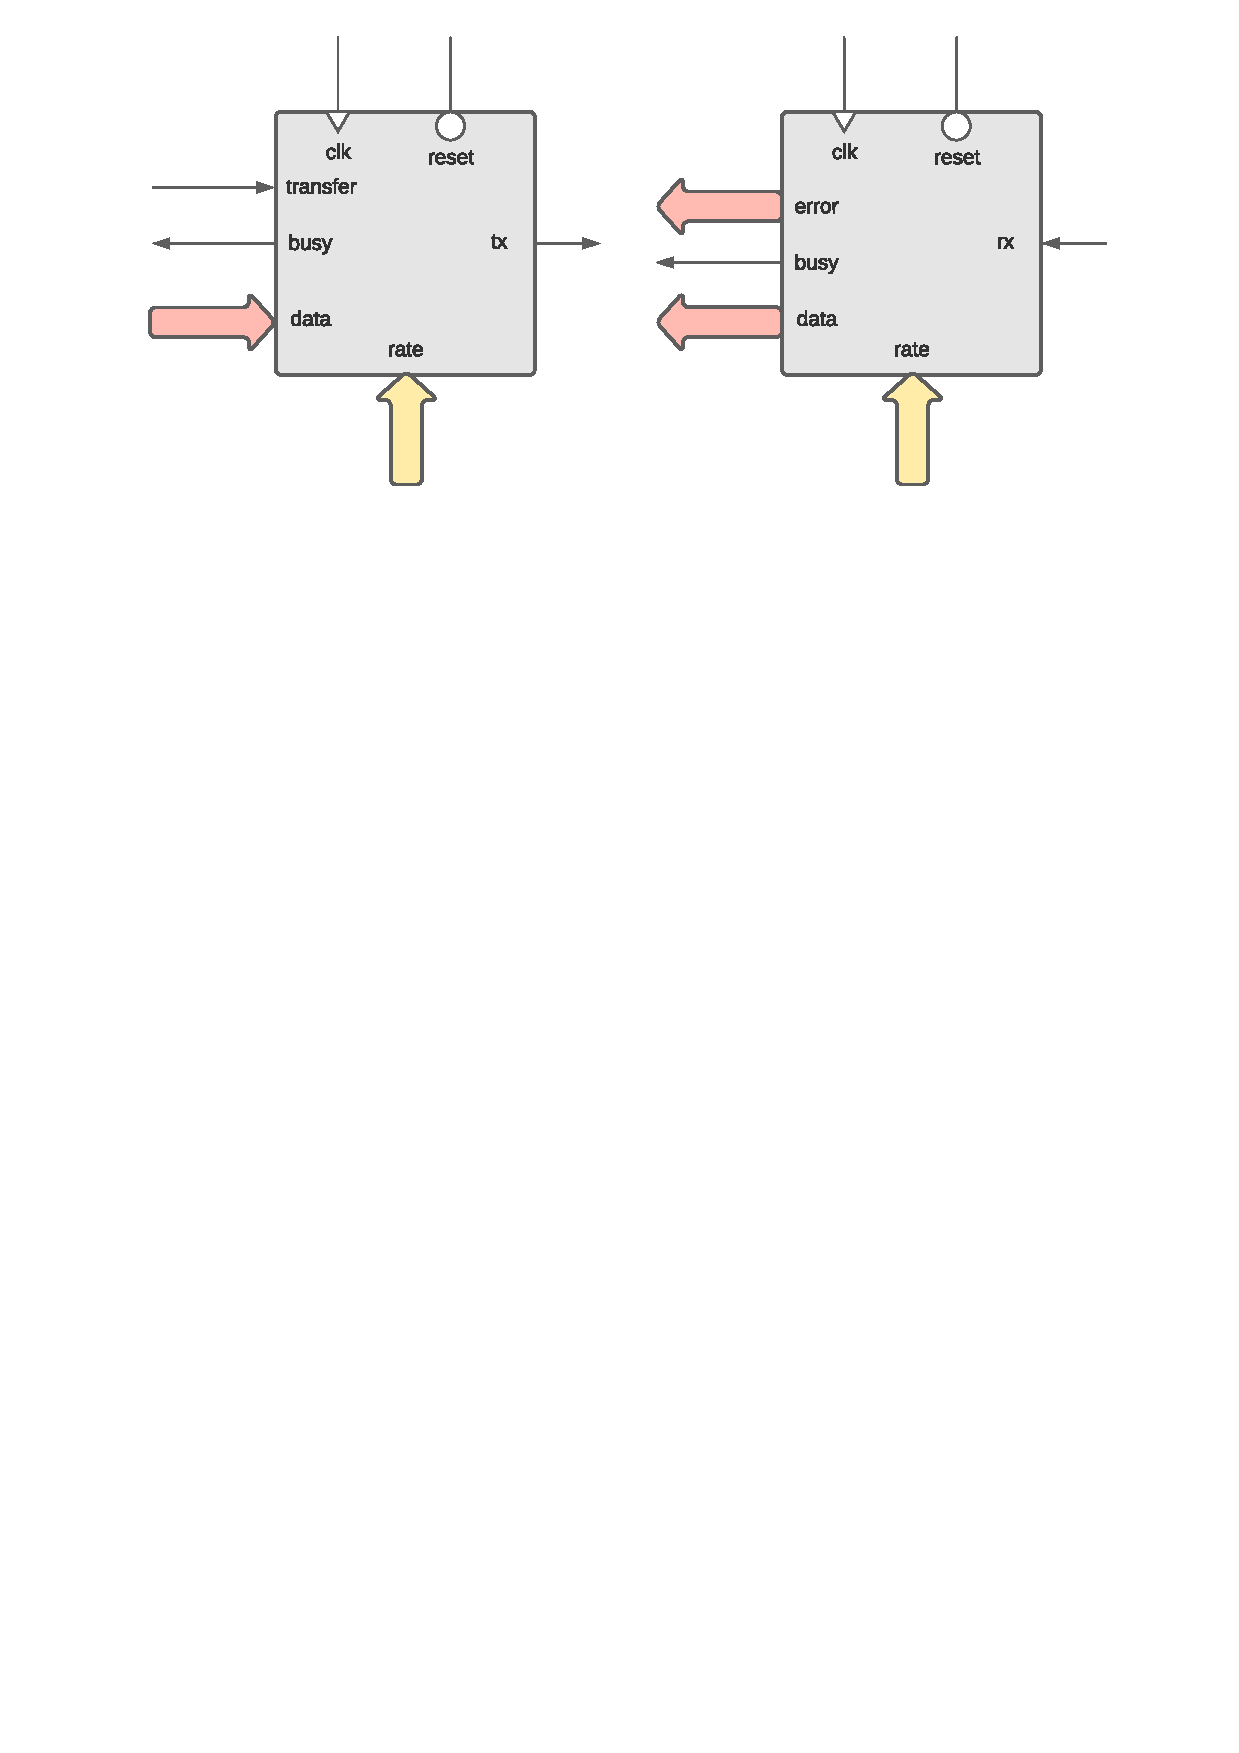
\includegraphics[scale=0.75]{img/diagrams/uart.pdf}
    \captionsetup{format=plain,justification=centering}
    \caption{Struktura wyprowadzeń modułów UART TX orax UART RX}
    \label{uart-structure}
\end{figure}
\vspace{0.5cm}

Struktury \verb|entity| reprezentujące obie podjednostki wyposarzono w~identczny zestaw parametrów (ang. \textit{generic}). Pozwalają one określić szerokość portu \verb|rate| i~format przesyłanych danych (liczbę bitów danych i~stopu oraz rodzaj parzystości). Przy ich pomocy możliwe jest też zanegowanie sygnału transmisyjnego tak, aby bezczynność linii transmisyjnej symbolizowana była stanem wysokim oraz (niezależne) zanegowanie bitów danych. W~projekcie wykorzystane zostały oba rodzaje negacji. 

Obie jednostki zostały zaimplementowane jako synchroniczne automaty skończone o~pięciu stanach. Pierwszy z~nich - \textit{idle} - przyjmowany jest w~momentach bezczynności, tj. gdy moduł oczekuje na wykrycie stanu aktywnego linii odbiorczej lub linii \verb|transfer|. W~momencie zajścia warunków startu automat przechodzi w~stan odbioru/transmisji bitu startu. Przy przejściu tym resetowany jest wewnętrzny licznik długości znaku oraz ustawiana jest linia \verb|busy|. Wartość znajdujące się na wejściu \verb|rate| zapisywana jest w~wewnętrznym buforze. W~przypadku transmisji zapisywana jest także wartość na wejściu \verb|data| a~stan linii \verb|tx| zmieniany jest na aktywny. Rzeczony licznik inkrementowany jest następnie o~jeden w~każdym następnym cyklu zegara systemowego. Moduł odbiorczy oczekuje aż jego wartość dojdzie do połowy zapisanej wartości \verb|rate| (powiększonej o~1), a~następnie próbkuje stan linii \verb|rx| w~celu zweryfikowania stanu bitu startu. Moduł nadawczy czeka natomiast czas dwukrotnie dłuższy. W~przypadku obu jednostek sytuacje te wiążą się z~przejściem do kolejnego stanu - odbioru/transmisji bitów danych. Przejście do wszystkich kolejnych stanów (odbioru/nadawania bitów danych, parzystości i~stopu) wiąże się ze zresetowaniem licznika długości trwania znaku. W~przypadku odbioru bitów startu, stopu oraz parzystości odbywa się także ewentualne ustawieniem odpowiedniej flagi błędu w~wewnętrznym buforze. Przejścia do kolejnych stanów wywoływane są osiągnięciem wartości \verb|rate| przez licznik. W~następnym cyklu po odebraniu/nadaniu wszystkich bitów, stan linii \verb|busy| ustawiany jest na niski, a~dane i~flagi błędu (w~przypadku odbioru) kopiowane są z~wewnętrznych buforów na wyjście.

Dla każdego modułu stworzona została symulacja mająca na celu zweryfikowanie poprawności działania. W~jej ramach zostały stworzone procedury biblioteczne realizujące niezależnie funkcjonalność transmisji/odbioru, których kod został oparty na materiałach udostępnionych w~trakcie wykładów. Posiłkowanie się nimi miało na celu eliminację potencjalnych błędów w~procesie weryfikacji.

\vspace{0.5cm}
\begin{figure}[ht]
    \centering
    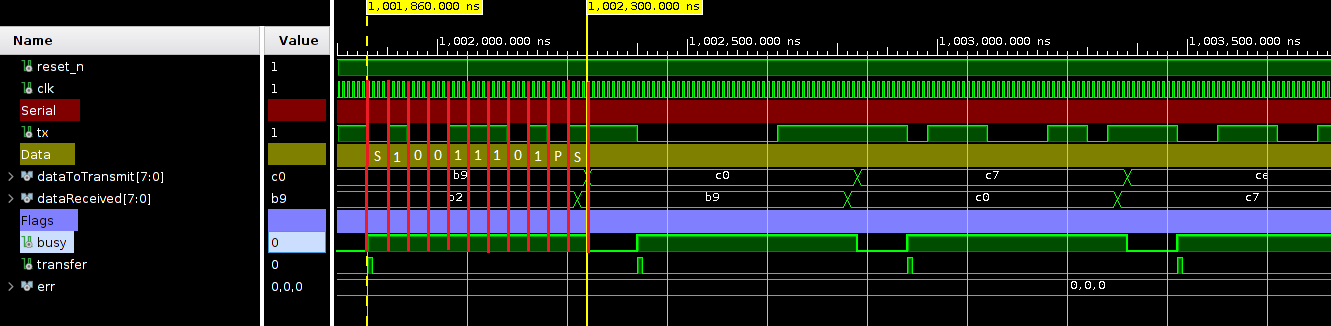
\includegraphics[scale=0.7]{img/sim/communication/uart_tx_sim.png}
    \captionsetup{format=plain,justification=centering}
    \caption{Wycinek sumylacji modułu UART TX}
    \label{sim-uart-tx}
\end{figure}
\vspace{0.5cm}

Symulacje miały charakter całościowy, tj. przetestowane zostały wszystkie kombinacje bitów transmitowanego słowa. Na Rys. \ref{sim-uart-tx} przedstawiono wycinek symulacji modułu TX. Transmitowane dane mają w~tym przypadku format 8E1. Prędkość transmisji to 25MHz natomiast prędkość zegara systemowego to 100MHz. Zastosowano tu zarówno negację sygnału jak i~danych. Pionowe linie w~kolorze czerwonym rozmieszczone zostały w~odstępach czterech cykli zegara systemowego, co odpowiada długości trwania transmitowanego bitu. Przedziadziały oznaczone literami S~odnszą się kolejno do bitu startu oraz bitu stopu. Zgodnie z~oczekiwaniami odpowiadający im stan linii \verb|tx| to odpowiednio niski i~wysoki. Bity danych to kolejno $10011101$. Po odwróceniu ich klejności (słowa transmitowane są w~kolejonści od najmniej do najbardziej znaczącego bitu) otrzymujemy $10111001$. Dane te zapisane w~formacie heksadecymalnym mają postać $0$x$B9$. Identyczna wartość ukazana jest na obrazie symulacji w~wierszu \verb|dataToTransmit|\footnote{Wysyłane słowo były wektorami losowymi z~realizacji rozkładu jednostajnego implementowanego za pomoca funkcji \textit{uniform} biblioteki \textit{math\_real}}, który obrazuje aktualnie transmitowane słowo. Oznacza to, że bity danych zostały nadane poprawnie. Bit parzystości ustawiony jest w~stanie niskim. Biorą pod uwagę nieparzystą liczbę jedynek w~przesyłanym słowie oraz negację sygnału i~danych można stwierdzić, że również ten bit został przesłany poprawnie. Sygnał \verb|dataReceived| jest ustawiany na wartość odebraną przez ww. funkcję biblioteczną. Jak widać, jego wartość zmienia się na oczekiwaną ($0$x$B9$) w~momencie połowy trwania bitu stopu. Na rysunku zaznaczone zostały także momenty ustawienia i~zresetowania stanu linii \verb|busy|. Różnica między nimi opiewa na $440$ ns. Jest to również wartość oczekiwana, ponieważ czas trwania pojedynczego bitu wynosi $40$ ns (cztery takty zegara systemowego) a~sumaryczna liczba transmitowanych bitów to $11$ ($1 + 8 + 1 + 1$). Aby ułatwić weryfikację działania modułu symulacja została zaprojektowana tak, aby w~momencie niezgodności odbieranego znaku z~sygnałem \verb|dataToTransmit| stan bitów linii \verb|dataReceived| ustawiany był na $X$ reprezentowany w~symulacji kolorem czerwonym.

\vspace{0.5cm}
\begin{figure}[ht]
    \centering
    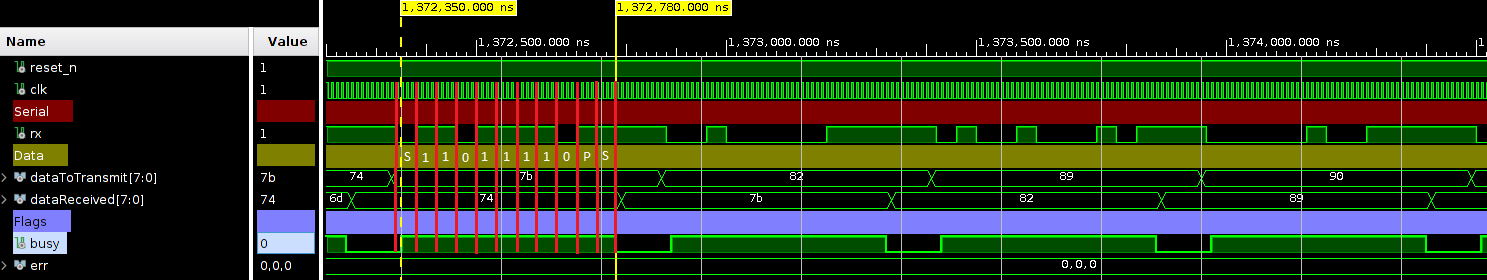
\includegraphics[width=\textwidth]{img/sim/communication/uart_rx_sim.png}
    \captionsetup{format=plain,justification=centering}
    \caption{Wycinek sumylacji modułu UART RX}
    \label{sim-uart-rx}
\end{figure}
\vspace{0.5cm}

Wycinek analogicznej symulacji dla modułu RX (przeprowadzonej przy tych samych parametrach transmisji) został zaprezentowany na Rys. \ref{sim-uart-rx}. Ponowienie analizy przeprowadzonej dla przypadku transmisji pozwala stwierdzić, że również odbiór danych odbywa się prawidłowo. Warto zauważyc, że czas wysoki na linii \verb|rx| trwa o~10 ns krócej, niż w~poprzednim przypadku. Wynika to z~faktu, że automat skończony modułu RX wychodzi ze stanu \textit{idle} dopiero w~momencie odczytania stanu aktywanego na linii odbiorczej\footnote{Po przygotowaniu grafik do sprawozdania zauważono, że moduł RX czeka o~jeden takt zegara za długo na wystawienie odberanych danych (które są gotowe już w~połowie trwania ostatniego bitu stopu). Błąd ten wynikał z~ustawienia niewłaściwego momentu próbkowania bitu startu, który przesuwał pozostałe chwile próbkowania. Został on poprawiony.}.

Przeprowadzone symulacje pozwoliły poprawić początkowe błędy implementacji a~tym samym przejść do kolejnego etapu projektowania interfejsu komunikacyjnego. Było nim stworzenie jednostek akumulujących odbierane i~transmitowane słowa do postaci N-bajto- wych próbek (określanych niżej mianem \textit{SampleTx} i~\textit{SampleRx}). Ich interfejs jest niemal identyczny jak ten przedstawiony na Rys. \ref{uart-structure}. Jedynymi różnicami są szerokość portów \verb|data| oraz brak portów wejściowych \verb|rate|. Szybkość transmisji jest w~ich przypadku ustalana poprzez parametry (\textit{generic}). Wzbogacają one interfejs UART o~dodatkowy N-bajtowy bufor wraz z~multiplekserem o~N~8-bitowych wejściach, którego wyjście połączone jest z~portem \verb|data| wewnętrznej instancji podjednostki UART TX/RX. Układy te pozwalają na odbiór/transmisję próbek w~formacie \textit{little endian} wybranym ze względu na wykorzystanie w~projekcie komputera opartego o~architekturę x86-64. Również w~ich przypadku zaprojektowane zostały symulacje mające na celu sprawdzenie poprawności dekompozycji słów na kolejno wysyłane/odbierane bajty. Filozofia ich działania jest również analogiczna do tej przedstawionej powyżej. Funkcjonalność komplementarna względem testowanego modułu jest implementowana poprzez wykonane wcześniej funkcje biblioteczne wzbogcone o~logikę pozwalającą operować na N-bajtowych słowach. Aktualnie wysyłane dane mogą być obserwowane na symulacji jako sygnał \textit{sampleToTransmit}, natomiast dane odebrane jako sygnał \textit{sampleReceived}. Jeden z~nich ustawiany jest zawsze przez moduł testowany, a~drugi przez proces wywołujący funkcję biblioteczną. Wycinek rzeczonych sumlacji dla przypadku $N=2$ został zaprezentowany na Rys. \ref{sim-sample-trensreceiver}. Niezgodność danych odbieranych z~danymi wysyłanymi lub błąd odbioru sygnalizowane są ponownie ustawieniem bitów sygnału \textit{sampleReceived} w~stan $X$.

\vspace{0.5cm}
\begin{figure}[ht]
    \centering
    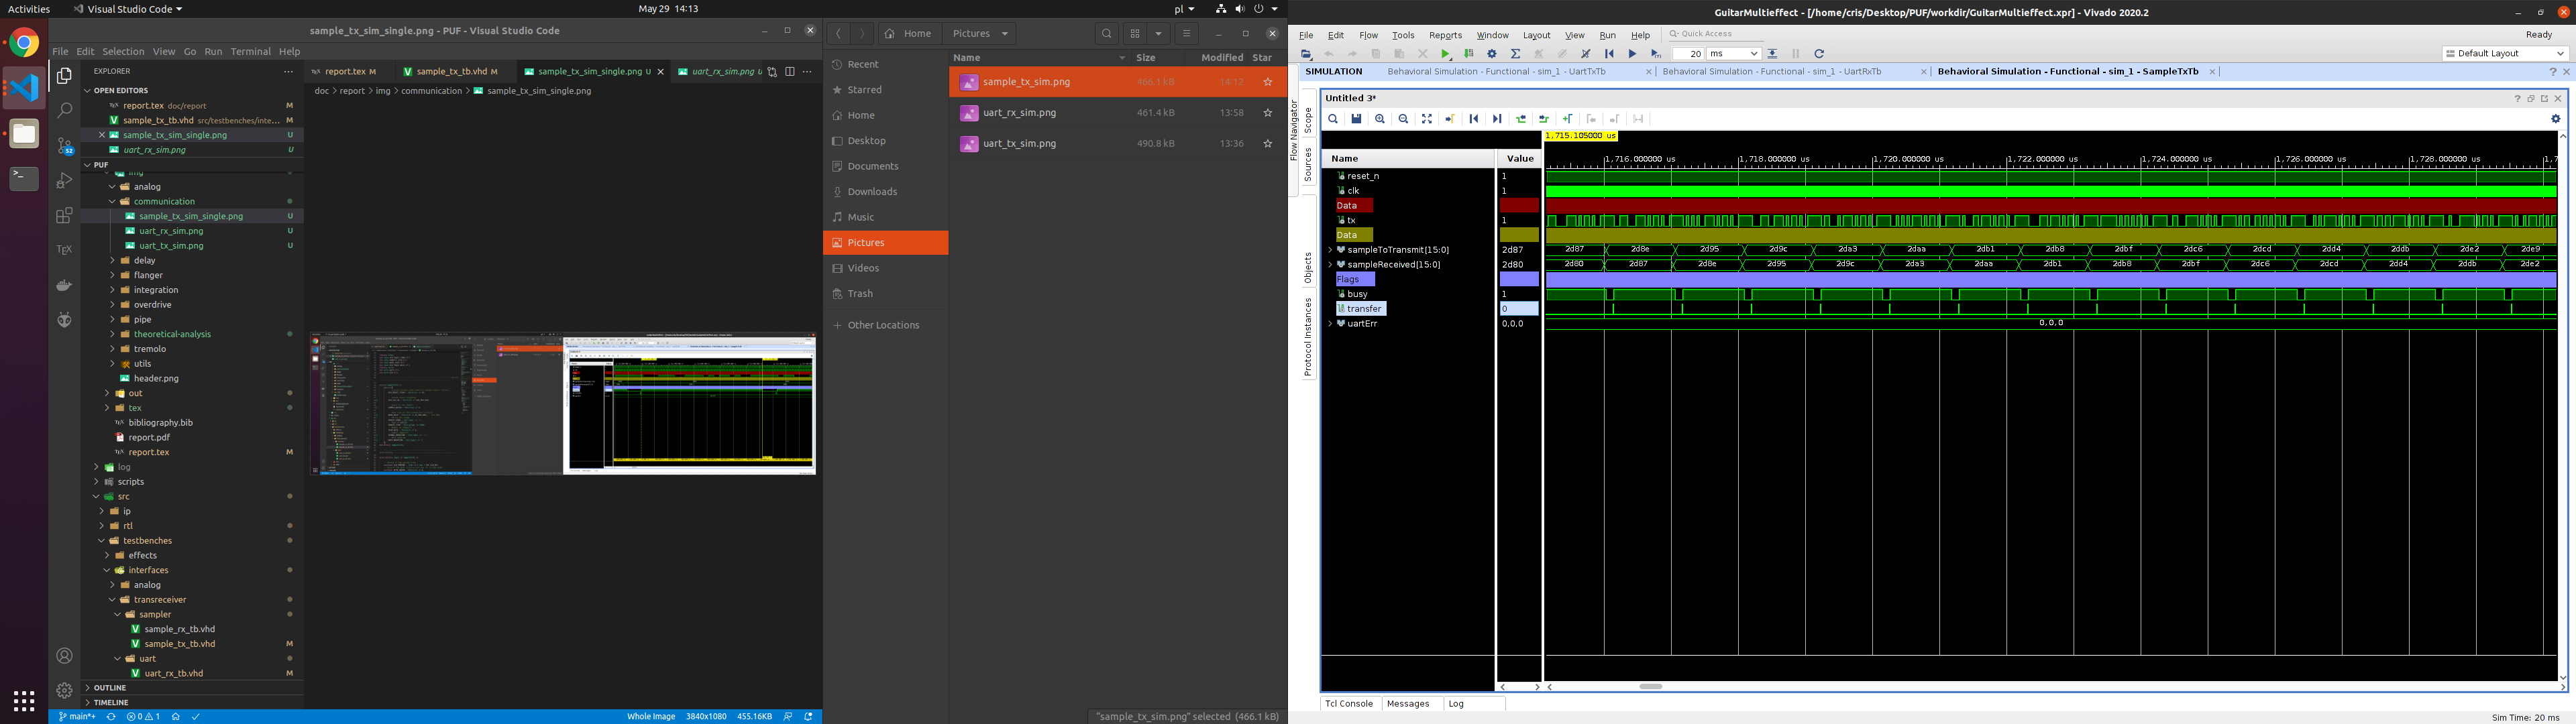
\includegraphics[width=\textwidth]{img/sim/communication/sample_tx_sim_multiple.png}
    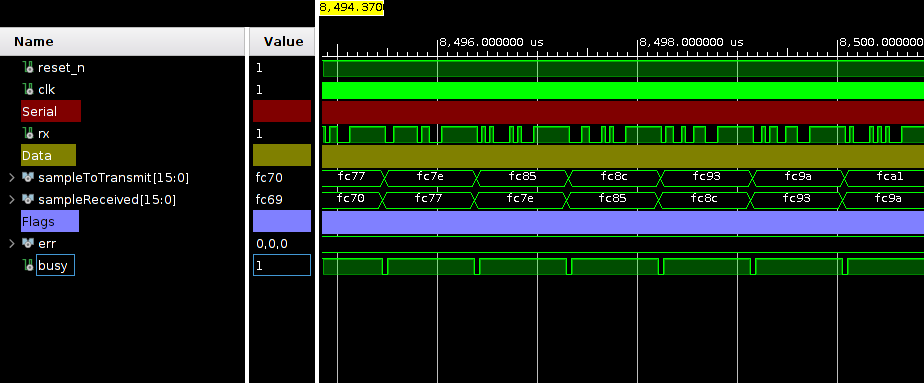
\includegraphics[width=\textwidth]{img/sim/communication/sample_rx_sim_multiple.png}
    \captionsetup{format=plain,justification=centering}
    \caption{Wycinek sumylacji modułów \textit{SampleTx} (u~góry) i~\textit{SampleRx} (u~dołu)}
    \label{sim-sample-trensreceiver}
\end{figure}
\vspace{0.5cm}
